\documentclass[11pt,a4paper]{article}


\usepackage[top=2cm, bottom=2cm, left=2cm, right=2cm]{geometry} %Margins if you run out of space

\usepackage[style=ieee]{biblatex}
\addbibresource{references.bib}

\usepackage[latin1]{inputenc}
\usepackage{amsmath}
\usepackage{amsfonts}
\usepackage{amssymb}
\usepackage{graphicx}
\usepackage{longtable}
\usepackage{array}

\usepackage{listings}
\usepackage{tikz}

\usepackage{enumitem}

\tikzset{main node/.style={circle,fill=blue!20,draw,minimum size=1cm,inner sep=0pt},
}

\usepackage{hyperref}
\hypersetup{allbordercolors=white, colorlinks=true, allcolors=blue}
%\addtokomafont{disposition}{\rmfamily}




\title{Model-Driven Engineering (MODE) Open Individual Assessment}
\author{Examination Number: Y1403115}
\date{}

\begin{document}
	
\maketitle

\section{Abstract Syntax and Constraints}
%Explain how you have arrived at the abstract
%syntax and any well-formedness constraints for your DSL, justify the decisions
%that you have made, and discuss how you have tested your abstract syntax and
%well-formedness constraints.

	\subsection{Problem analysis}
	A domain specific language (DSL) needs to be defined which allows the creation, modification and modelling relationships between four entities - system requirements, customer requirements, team members and test-cases. Possible relationships between two requirements can be decomposition(also referred to as dependency in this report) and conflict. Requirements can be assigned to team members and can also be verified by test-cases. 
	The implementation of the metamodel in Emfatic defines 4 concrete classes for each of the entities mentioned above along with a container class RequirementsModel and a few abstract classes defined to limit duplication and enforce constraints.
	
	\begin{lstlisting}
	class RequirementsModel
	abstract class Identifiable
	abstract class Describable
	abstract class Requirement extends Identifiable, Describable
	class CustomerRequirement extends Requirement
	class SystemRequirement extends Requirement
	class TestCase extends Identifiable, Describable
	class TeamMember extends Identifiable
	\end{lstlisting}
	
	\subsection{Abstract classes}
	System requirements and customer requirements share a number of common properties. It is obvious that having a super class Requirement, which captures these common properties is beneficial and avoids duplication. All requirements have a progress attribute and an updateProgress operation which will be discussed later on.
	
	According to the specification, both requirements and test-cases need to have a description. This is a string attribute in terms of the Emfatic code. In order to avoid duplication by defining this attribute in both classes an abstract class Describable is used, which is a superclass of both requirements and test-cases. An additional constraint for requirement description is that they need to be at least 10 characters long. This is enforced via the EVL \cite{kolovos2010} validation.
	
	Requirements also must have an unique identifier. While not specifically stated in the specification, being able to uniquely identify test-cases and team members is an important property of the DSL, as it avoids visual ambiguity for users. For this reason, the abstract class Identifiable is defined, which has a string attribute id, and is a super class of requirements, test-cases and team members. The uniqueness constraint is enforced by the EVL validation.
	
	\subsection{Requirement Decomposition}
	Requirements are the most important entities in the DSL. They form a directed acyclic graph structure of decomposition relationships. For simplicity a parent-child abstraction is used to model this relationship. That is requirements being decomposed are parents of requirements in the decomposition and the latter are children of the former. The decomposition relationships can be viewed as breaking down requirements into multiple smaller child requirements, which together form the parent requirement. This must be true because, according to the specification, parent requirement's progress is the average of it's children, which is 100\% when all of it's children are also 100\%. Further constraints on this realationship are:
	
	\begin{enumerate}[noitemsep] \label{lst:constraints}
		\item Customer requirements can be decomposed into technical requirements, but not the other way round.
		\item Each customer requirement needs to be decomposed into at least one technical requirement.
		\item Each technical requirement needs originate from at least one customer requirement.
		\item Requirements decomposition must be free of cycles.
	\end{enumerate}
	
	This means that each path in the requirements graph (see \autoref{fig:graph}) must begin with 1 or more customer requirements followed by 1 or more system requirements. The metamodel defines a ref
	
	\begin{figure}[h!]
		
		\centering
	
		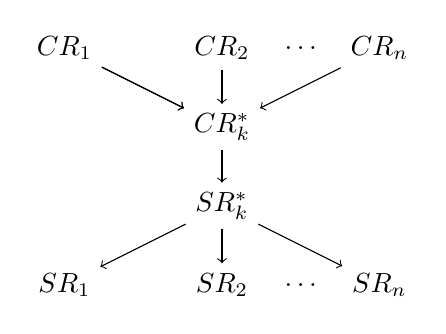
\begin{tikzpicture}
		
			\node (a) at (0,3)  {$CR_1$};
			\node (b) at (2,3)  {$CR_2$};
			\node (c) at (3,3)  {$\ldots$};
			\node (d) at (4,3)  {$CR_n$};
			
			\node (e) at (2,2)  {$CR_k^{*}$};
			
			\node (f) at (2,1)  {$SR_k^*$};
			
			\node (g) at (0,0)  {$SR_1$};
			\node (h) at (2,0)  {$SR_2$};
			\node (i) at (3,0)  {$\ldots$};
			\node (j) at (4,0)  {$SR_n$};
			
			\draw (a) edge[->] (e) 
			(a) edge[->] (e)
			(b) edge[->] (e)
			(d) edge[->] (e)
			(e) edge[->] (f)
			(f) edge[->] (g)
			(f) edge[->] (h)
			(f) edge[->] (j);
			
		\end{tikzpicture}
		
		\caption{Requirement graph structure}
		\label{fig:graph}
	\end{figure}	

	To model this relationship in the Emfatic code the Requirements superclass has a multivalued reference of type Requirement, for both the children and parents of the requirement. All of the constraints discussed above are handled by the model validation in EVL.
	
	An alternative solution is to have the children and parent references in the subclasses as shown on \autoref{fig:alt-req}. This way system requirements are restricted to have only system requirements as children. However an opposite for systemParents has to be both customerChildren and systemChildren, which is not possible in Ecore and being able to navigate from children to parents as well as the other way around is very important for the model management tasks. So this solution was ultimately discounted.
	
	\begin{figure}[h!]
	\centering
	\begin{lstlisting}
class CustomerRequirement extends Requirement{
	ref Requirement[*]#conflictsIncoming customerChildren;
	ref CustomerRequirement[*] customerParents;
}
	
class SystemRequirement extends Requirement{
	ref SystemRequirement[*]#systemParents systemChildren;
	ref Requirement[*] systemParents;
}
	\end{lstlisting}
	
	\caption{Alternative implementation of requirements decomposition.}
	\label{fig:alt-req}
	
	\end{figure}
	

	\subsection{Requirement Conflicts}
	Requirements can also be in conflict with each other, which means that only one of them can be completed. Conflicts are constrained to the same type of requirement - system requirements can be in conflict with system requirements only and customer requirements with customer requirements only. This constraint is directly enforced by the meta-model by having different types for the conflicts reference. It is also important to be able to navigate both ways of a conflict relation ship and this is why opposites are used as well. 
	
	Additional constraints on conflicts arise from the nature of requirement decomposition and progress and are defined in the EVL validation. It does not make sense for requirements to decompose into requirements, with which they are in conflict. Also the decompositions of two conflicting requirements must be two disjoint sets of requirements otherwise one of them would not be completable without the other. Even when having these constraints users are still able to mark two conflicting requirements as complete, which should not be possible. This is way an additional EVL constraint is defined which checks if two conflicting requirements are both complete.
	
	\subsection{Requirement Progress}
	All requirements have a progress field which is either set by the user, if the requirement doesn't have any children or is the average of it's children?s progress. An easy way to enforce this constraint on the progress field is to leave it to the user to calculate the progress of each requirement and just check weather or not the constraint is satisfied in the EVL validation. However this is very error prone and not user friendly. 
	
	In order to automate calculation of progress, the java code of the GMF editor had to be modified. In particular the RequirementImpl.java file which defines the implementation of requirement entities. An updateProgress method is defined which calculates progress of a requirement from the progress of it's children (taking the average). Whenever a requirement's progress is set by the user  updateProgress method on all of it's parents and whenever a requirement is assigned a new child it recalculates it's own progress again notifying parents of the change. Also whenever the progress of a parent requirement is set manually it automatically calculates the correct average progress of it's children and ignores the user defined progress. This is done using the notification mechanism of EMF \cite{emf} - by adding an adapter to the requirement which listenes to SET notifiactions for progress and children fields. 
	
	The more commonly used derived attributes pattern could not be used, as progress is a derived attribute only if the requirement has children and is user defined if it does not. 
	
	An EVL constrained is used to check that progress is a valid percentage - between 0\% and 100\%
	
	\subsection{Team Members and Test-cases}
	Leaf requirements in the requirements decomposition graph make up all of the work needed to complete the whole graph, because if they are 100\% complete, then all of their parents are also 100\% complete. This means it only ever makes sense for team members to work on leaf requirements and for test-cases to only verify leaf requirements. This is why EVL constraints defined for both test-cases and team members verify that only leaf requirements are assigned to any of them. 
	
	Altough, this approach complies with the assessment specification, assigning non-leaf requirements to team members and test-cases could provide better user experience. For example if all the children of a particular requirement are assigned to a specific team member, then it would be safe to indicate this by assigning the parent requirement to the team member instead. This would limit the number of connections in the visual editor and avoid visual ambiguity. And the same applies to test-cases. However, due to timing constraints on the assessment, this was not implemented.
	
	Another important constraint for test-cases to note is that they can verify only system requirements and this is enforced by the meta-model.
	
	\subsection{EVL Constraints}
	All EVL constraints have a sensible error message for the user. All except for the constraint that checks for cycles in the decomposition graph and the one that checks for the length of requirement descriptions also define a quick fix. The two constraints that do not have quick fixes defined, do not have a simple solution - it doesn't make sense to automatically generate a description if it is not long enough and fixing cycles in a graph is not straightforward at all. 
	
	\subsection{Testing}
	In order to test the abstract syntax and constraints, five simple example models were used. Each model tests a different aspect of the constraints.
	
	\begin{enumerate}[noitemsep]
		\item 1.Y1403115 - Tests requirement decomposition (dependencies).
		\item 2.Y1403115 - Tests id's, requirement description length and progress.
		\item 3.Y1403115 - Tests requirement conflicts.
		\item 4.Y1403115 - Tests test-cases.
		\item 5.Y1403115 - Tests team members.
	\end{enumerate}
	
	Each example model contains a correct graph of objects (whose names start with "Correct") and also several incorrect ones (whose names start with "Error"). Together all the models demonstrate all of the constraint failure cases. The example models were incrementally changed during development, as new issues arouse. 
	
	

	\section{Editor}
	%Explain the editor for your DSL, justify the decisions that you have made,
	%and briefly argue why your editor provides an appropriate notation for your DSL.
	
	\subsection{Description}
	The editor for the DSL is an Eugenia \cite{eugenia} generated GMF \cite{gmf} diagram editor. It uses a graph based diagram notation and it provides four types of nodes (objects) - CustomerRequirements, SystemRequirements, TeamMembers and TestCases. Each type of object has a different colour border in order to avoid visual ambiguity. All attributes of each object are editable from the text fields in the diagram.
	
	There are also different types of conncections between objects. The Dependency connection is an arrow, which indicates requirement decomposition relationship and the arrow points to the child requirement. System Requirement and Customer Requirement Conflicts are connections that indicate conflicts between the particular type of requirements and are represented by a dashed line with the same color as the requirement type. Verification and Assignment connections are used to relate requirements and team members and requirements and test-cases and have the same color as the particular object(team member or test-case).
	
	
	\subsection{Justification}
	The editor allows users to create and modify the fields of each type of the four main entities - system and customer requirements, test-cases and team members. All references between the entities can be modelled using connections. And the color coding makes models much clearer and easier to understand.



	\section{Model Management Operations}
	%Explain the model management operations for
	%your DSL, justify the decisions that you have made, and briefly demonstrate that
	%the model management operations can be used to fulfill the model management
	%tasks described in Section 1.	
	
	\subsection{Model to Model Transformation}
	The M2M (Model to Model) transformation is done using the Epsilon Transformation Language (ETL) \cite{etl} and is done in a single ETL file. It takes an imput model and creates an output model removing all completed requirements. Following the ETL syntax rules are defined for transforming each object in the input model to a coresponding object in the output model. The requirements transformation rule uses a guard in order to create requirements in the output model only if they are not completed. In the same rule also the children and parents for each requirement are filtered so that only non completed ones exist in the output model. Team members and test-cases are transformed only if they contain at least one non completed requirement. Because there are several abstract classes defined in the meta model it makes sense to use the concept of abstract transformation rules from ETL to transform them. This limits duplication in the M2M transformation rules.
	
	\subsubsection{Running Instructions}
	The M2M transformation can be ran using an ETL eclipse run configuration, which specifies and input model named "In" and an output model named "Out".
	
	\subsection{Model to Text Transformation}
	The model to text transformation is (M2T) transformation is implemented in the Epsilon Generation Language \cite{egl} and is split across multiple EGL files:
	\begin{itemize}[noitemsep]
		
		\item requirement2page.egl - Generates an html page from a requirement.
		\item teamMember2page.egl  - Generates an html page from a team member.
		\item testCase2page.egl - Generate an html page from a test-case
		\item model2index.egl - Generate main html page from requirementsModel.
		\item util.egl - Some utility functiions used to create links, lists of objects and nested list of requirements.
		\item main.egl - Coordinates the generation of all pages for a particular model. Uses input parameters so it can be reused for generating different versions of the same website.
		\item Y1403115.xml - ANT \cite{ant} build xml file, which generates a simplified model from the original one and then generates two versions of the website - one for the original and one for the simplified model and links them together.
	\end{itemize}

	The most complex requirement for the M2T transformation is the ability to filter out completed requirements. This is done by generating two versions of the website - one with all requirements and one with non completed requirements only. Every page of both websites links to the main page of the other. In order to generate the simplified version of the website the M2M transformation described in the previous chapter is used. This is common model driven engineering pattern, which separates the simplification of the model from the generation of the text and also avoids duplication of the M2M functionality in the M2T transformation. In order to create a single version of the website the main.egl script requires some parameters in order to create the links to the other website version. These parameters are the suffix appended to all page names, the suffix of the other version of the website and the text to display in the cross-reference link. Each page in the website uses the id of the object it represents as the file name (along with the version suffix), this can be done since id's always need to be unique. In order to ensure that the original model used for the M2T transformation is valid the EVL validation is also part of the ant build task.
	
	The index page of each version of the website shows the requirements graph as a nested list of links. Followed by test-cases and their corresponding requirements and then team members and their coresponding requirements. 
	
	In order to drill down the requirements/test-cases decomposition tree a user can navigate requirements pages by following links to their children and/or test-cases. 
	
	The progress of each requirement is shown as a progress bar on each requirements page.

	\subsubsection{Running Instructions}
	The transformation can be ran from the Y1403115.xml ANT build script. The transformed model has to be specified manually in the script. Also the locations of the m2m transformation folder and the Y1403115.evl valiation script are hard coded in the build script as well as the output directory which is created in the same folder as the build script and is called "gen". Also in order for eclipse to pick up changes in the gen directory it has to be manually refreshed.
	
\printbibliography

\end{document}
